\UseRawInputEncoding
\documentclass[a4paper, 14pt]{extarticle}

% Поля
%--------------------------------------
\usepackage{geometry}
\geometry{a4paper,tmargin=2cm,bmargin=2cm,lmargin=3cm,rmargin=1cm}
%--------------------------------------


%Russian-specific packages
%--------------------------------------
\usepackage[T2A]{fontenc}
\usepackage[utf8]{inputenc} 
\usepackage[english, main=russian]{babel}
\usepackage{cmap}
%--------------------------------------

\usepackage{textcomp}

% Красная строка
%--------------------------------------
\usepackage{indentfirst}               
%--------------------------------------             


%Graphics
%--------------------------------------
\usepackage{graphicx}
\graphicspath{ {./images/} }
\usepackage{wrapfig}
%--------------------------------------

% Полуторный интервал
%--------------------------------------
\linespread{1.3}                    
%--------------------------------------

%Выравнивание и переносы
%--------------------------------------
% Избавляемся от переполнений
\sloppy
% Запрещаем разрыв страницы после первой строки абзаца
\clubpenalty=10000
% Запрещаем разрыв страницы после последней строки абзаца
\widowpenalty=10000
%--------------------------------------

%Списки
\usepackage{enumitem}

%Подписи
\usepackage{caption} 

%Гиперссылки
\usepackage{hyperref}

\hypersetup {
	unicode=true
}

%Рисунки
%--------------------------------------
\DeclareCaptionLabelSeparator*{emdash}{~--- }
\captionsetup[figure]{labelsep=emdash,font=onehalfspacing,position=bottom}
%--------------------------------------

\usepackage{tempora}
\usepackage{amsmath}
\usepackage[dvipsnames]{xcolor}
\usepackage{listings}
\lstset{
  belowcaptionskip=1\baselineskip,
  breaklines=true,
  frame=L,
  xleftmargin=\parindent,
  language=Java,
  showstringspaces=false,
  basicstyle=\footnotesize\ttfamily,
  keywordstyle=\bfseries\color{blue},
  commentstyle=\itshape\color{purple},
  identifierstyle=\color{black},
  stringstyle=\color{red},
  numbers=left,           
  numberstyle=\tiny\color{gray}, 
  numbersep=10pt,      
  % ------------------------------
}

%--------------------------------------
%			НАЧАЛО ДОКУМЕНТА
%--------------------------------------

\begin{document}

%--------------------------------------
%			ТИТУЛЬНЫЙ ЛИСТ
%--------------------------------------
\begin{titlepage}
\thispagestyle{empty}
\newpage


%Шапка титульного листа
%--------------------------------------
\vspace*{-60pt}
\hspace{-65pt}
\begin{minipage}{0.3\textwidth}
\hspace*{-20pt}\centering

\includegraphics[width=\textwidth]{emblem}
\end{minipage}
\begin{minipage}{0.67\textwidth}\small \textbf{
\vspace*{-0.7ex}
\hspace*{-6pt}\centerline{Министерство науки и высшего образования Российской Федерации}
\vspace*{-0.7ex}
\centerline{Федеральное государственное бюджетное образовательное учреждение }
\vspace*{-0.7ex}
\centerline{высшего образования}
\vspace*{-0.7ex}
\centerline{<<Московский государственный технический университет}
\vspace*{-0.7ex}
\centerline{имени Н.Э. Баумана}
\vspace*{-0.7ex}
\centerline{(национальный исследовательский университет)>>}
\vspace*{-0.7ex}
\centerline{(МГТУ им. Н.Э. Баумана)}}
\end{minipage}
%--------------------------------------

%Полосы
%--------------------------------------
\vspace{-25pt}
\hspace{-35pt}\rule{\textwidth}{2.3pt}

\vspace*{-20.3pt}
\hspace{-35pt}\rule{\textwidth}{0.4pt}
%--------------------------------------

\vspace{1.5ex}
\hspace{-35pt} \noindent \small ФАКУЛЬТЕТ\hspace{80pt} <<Информатика и системы управления>>

\vspace*{-16pt}
\hspace{47pt}\rule{0.83\textwidth}{0.4pt}

\vspace{0.5ex}
\hspace{-35pt} \noindent \small КАФЕДРА\hspace{50pt} <<Теоретическая информатика и компьютерные технологии>>

\vspace*{-16pt}
\hspace{30pt}\rule{0.866\textwidth}{0.4pt}
  
\vspace{11em}

\begin{center}
\Large {\bf Лабораторная работа № 6} \\ 
\large {\bf по курсу <<Языки и методы программирования>>} \\ 
\large <<Программа с графическим пользовательским 
интерфейсом>>
\end{center}\normalsize

\vspace{8em}


\begin{flushright}
  {Студент группы ИУ9-21Б Воронков А. С.\hspace*{15pt} \\
  \vspace{2ex}
  Преподаватель Посевин Д. П.\hspace*{15pt}}
\end{flushright}

\bigskip

\vfill
 

\begin{center}
\textsl{Москва 2026}
\end{center}
\end{titlepage}
%--------------------------------------
%		КОНЕЦ ТИТУЛЬНОГО ЛИСТА
%--------------------------------------

\renewcommand{\ttdefault}{pcr}

\setlength{\tabcolsep}{3pt}
\newpage
\setcounter{page}{2}

\section{Цель}\label{Sect::task}
\par 
Приобретение навыков разработки программ с графическим пользовательским 
интерфейсом на основе библиотеки swing.   
\section{Задание}
В течение лабораторной работы нужно разработать программу, рисующую на экране:
\begin{itemize}
    \item Треугольник, заданный сторонами a, b и c,
    закрашенный цветом, компоненты R, G и B
    которого зависят от величины углов
    треугольника (угол 0 соответствует величине 0
    компоненты, а угол 180 – величине 255).
 
    \item Прямоугольник, заданный сторонами a и b,
    изображённый таким образом, что его длинная
    сторона составляет угол альфа с осью OX.


\end{itemize}

\pagebreak
\section{Практическая реализация}
\par
Код файла PictureForm.java
\begin{lstlisting}
import javax.swing.*;
import javax.swing.event.ChangeEvent;
import javax.swing.event.ChangeListener;

public class PictureForm {
    private JPanel mainPanel;
    private JTextField areaField;
    private JSpinner radiusSpinner;
    private CanvasPanel canvasPanel;
    private JSpinner aSpinner;
    private JSpinner bSpinner;
    private JSpinner cSpinner;
    private JTextPane xtext;
    private JTextPane ytext;
    private JTextPane ztext;

    public void setXYZText() {
        xtext.setText(String.format("%d градусов", canvasPanel.getAngleX()));
        ytext.setText(String.format("%d градусов", canvasPanel.getAngleY()));
        ztext.setText(String.format("%d градусов", canvasPanel.getAngleZ()));
    }

    public PictureForm() {
        aSpinner.setValue(20);
        bSpinner.setValue(20);
        cSpinner.setValue(20);
        setXYZText();
        aSpinner.addChangeListener(new ChangeListener() {
            @Override
            public void stateChanged(ChangeEvent e) {
                    int a = (int)aSpinner.getValue();
                    canvasPanel.setA(a);
                    setXYZText();
            }
        });
        bSpinner.addChangeListener(new ChangeListener() {
            @Override
            public void stateChanged(ChangeEvent e) {
                int b = (int)bSpinner.getValue();
                canvasPanel.setB(b);
                setXYZText();
            }
        });
        cSpinner.addChangeListener(new ChangeListener() {
            @Override
            public void stateChanged(ChangeEvent e) {
                int c = (int)cSpinner.getValue();
                canvasPanel.setC(c);
                setXYZText();
            }
        });
    }

    public static void main (String[ ]  args) {
        JFrame frame = new JFrame("Треугольник");
        frame.setContentPane (new PictureForm().mainPanel);
        frame.setDefaultCloseOperation(JFrame.EXIT_ON_CLOSE);
        frame.pack();
        frame.setVisible(true);
    }
}
\end{lstlisting}
\par
Код файла CanvasPanel.java
\begin{lstlisting}
import javax.swing.*;
import java.awt.*;
import java.lang.Math;

public class CanvasPanel extends JPanel {
    private int a = 20;
    private int b = 20;
    private int c = 20;
    private double x = Math.PI / 3;
    private double y = Math.PI / 3;
    private double z = Math.PI / 3;
    public void setA(int a) {
        this.a = a;
        recalcAngles();
        repaint();
    }
    public void setB(int b) {
        this.b = b;
        recalcAngles();
        repaint();
    }
    public void setC(int c) {
        this.c = c;
        recalcAngles();
        repaint();
    }
    public int getAngleX() { return (int)Math.toDegrees(x); }
    public int getAngleY() { return (int)Math.toDegrees(y); }
    public int getAngleZ() { return (int)Math.toDegrees(z); }

    private void recalcAngles() {
        if (a + b <= c || a + c <= b || b + c <= a) return;
        x = Math.acos((a * a + b * b - c * c) / (2.0 * a * b));
        y = Math.acos((a * a + c * c - b * b) / (2.0 * a * c));
        z = Math.PI - x - y;
    }
    protected void paintComponent(Graphics g) {
        super.paintComponent(g);

        if (a + b <= c || a + c <= b || b + c <= a) {
            g.drawString("Нельзя построить", 10, 20);
            return;
        }

        g.setColor(new Color((250 * getAngleX() / 180),
                (250 * getAngleY() / 180),
                (250 * getAngleZ() / 180)));


        int cx = getWidth() / 2;
        int cy = getHeight() / 2;
        int[] xpoints = {cx - a/2, cx + a/2, cx  - a/2 + (int)(b * Math.cos(x))};
        int[] ypoints = {cy, cy, cy - (int)(b * Math.sin(x))};
        g.fillPolygon(xpoints, ypoints, 3);
        g.drawPolygon(xpoints, ypoints, 3);
    }
}
\end{lstlisting}
\par
Код файла PictureFrom2.java
\begin{lstlisting}
import javax.swing.*;
import javax.swing.event.ChangeEvent;
import javax.swing.event.ChangeListener;

public class PictureForm2 {
    private JPanel mainPanel;
    private JSpinner aSpinner;
    private JSpinner bSpinner;
    private JSpinner alphaSpinner;
    private CanvasPanel2 canvasPanel2;

    public PictureForm2() {
        aSpinner.setValue(20);
        bSpinner.setValue(40);
        alphaSpinner.setValue(45);
        aSpinner.addChangeListener(new ChangeListener() {
            @Override
            public void stateChanged(ChangeEvent e) {
                int a = (int)aSpinner.getValue();
                canvasPanel2.setA(a);
            }
        });
        bSpinner.addChangeListener(new ChangeListener() {
            @Override
            public void stateChanged(ChangeEvent e) {
                int b = (int)bSpinner.getValue();
                canvasPanel2.setB(b);
            }
        });
        alphaSpinner.addChangeListener(new ChangeListener() {
            @Override
            public void stateChanged(ChangeEvent e) {
                int alpha = (int)alphaSpinner.getValue();
                canvasPanel2.setAlpha(alpha);
            }
        });
    }

    public static void main(String[] args) {
        JFrame frame = new JFrame("Прямоугольник");
        frame.setContentPane (new PictureForm2().mainPanel);
        frame.setDefaultCloseOperation(JFrame.EXIT_ON_CLOSE);
        frame.pack();
        frame.setVisible(true);
    }
}
\end{lstlisting}
\par
Код файла CanvasPanel2.java
\begin{lstlisting}
import javax.swing.*;
import java.awt.*;
import java.lang.Math;

public class CanvasPanel2 extends JPanel{
    private int a = 20;
    private int b = 40;
    private int alpha = 45;
    public void setA(int a) {
        this.a = a;
        repaint();
    }
    public void setB(int b) {
        this.b = b;
        repaint();
    }
    public void setAlpha(int alpha) {
        this.alpha = alpha;
        repaint();
    }

    public int newX(int x, int y) {
        double alph = -Math.toRadians(alpha);
        return (int)Math.round(x * Math.cos(alph) - y * Math.sin(alph));
    }

    public int newY(int x, int y) {
        double alph = -Math.toRadians(alpha);
        return (int)Math.round(x * Math.sin(alph) + y * Math.cos(alph));
    }

    protected void paintComponent (Graphics g) {
        super.paintComponent (g);

        if (a < 0 || b < 0) {
            g.drawString("Нельзя построить", 10, 20);
            return;
        }

        g.setColor(Color.RED);

        int cx = getWidth() / 2;
        int cy = getHeight() / 2;
        int bigger;
        int lower;
        bigger = Math.max(a, b);
        lower = Math.min(a, b);
        int[] xpoints = {cx + newX(-bigger/2, -lower/2), cx + newX(bigger/2, -lower/2),
                cx + newX(bigger/2, lower/2), cx + newX(-bigger/2, lower/2)};
        int[] ypoints = {cy + newY(-bigger/2, -lower/2), cy + newY(bigger/2, -lower/2),
                cy + newY(bigger/2, lower/2), cy + newY(-bigger/2, lower/2)};

        g.drawPolygon(xpoints, ypoints, 4);
    }
}
\end{lstlisting}

\section{Результаты}
В результате лабораторной работы были созданы GUI приложения для визуализации геометрических фигур

\begin{center}
    \nopagebreak
    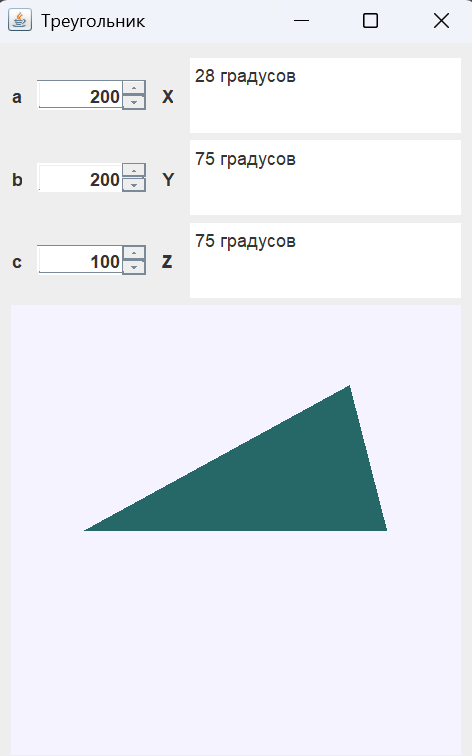
\includegraphics[width=0.85\textwidth]{lab6_1}
    \captionsetup{justification=centering}
    \captionof{figure}{Визуализация треугольника}
    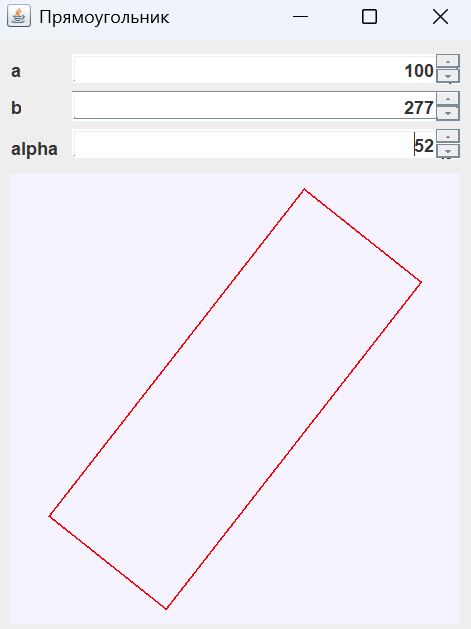
\includegraphics[width=0.85\textwidth]{lab6_2}
    \captionsetup{justification=centering}
    \captionof{figure}{Визуализация прямоугольника}
\end{center}

\section{Вывод}
В данной лабораторной работе были получены навыки работы модулем swing для реализации собственных GUI приложений
\end{document}